\section{Logika (back-end)}
\label{Chapter66}

Jednym z zadań w ramach pracy było zaprogramowanie odpowiedniej logiki biznesowej rozwiązującej zadania stawiane przed zaprojektowanym systemem. Najważniejszym zadaniem z perspektywy back-end'u jest interakcja z bazą danych. Poza tym system posiada: procesor zadań wykonywanych w tle oparty na \emph{cron}; moduły odpowiadające za komunikację z systemami uczelanianymi \emph{ePoczta} i \emph{eDziekanat}; moduł logowania zdarzeń. W trakcie implementacji zdecydowano się nie tworzyć osobnego mechanizmu do przechowywania ustawień w bazie danych i skorzystaliśmy z istniejącego już w \emph{Moodle}. Jednym z wymagań pozafunkcjonalnych było wykorzystanie bazy danych \emph{PostgreSQL}. Platforma \emph{Moodle} korzysta z mechanizmu \emph{XMLDB}, co pozwala na ominięcie wielu problemów pojawiających się przy migracjach pomiędzy różnymi systemami baz danych. Niestety kosztem wykorzystania tego mechanizmu jest konieczność pracy z interfejsami programowania aplikacji dostarczanym przez platformę \emph{Moodle} -- \emph{Data manipulation API}. Na diagramie poniżej znajdują się także klasy przechowujące stałe: (\emph{tables}, \emph{settings}.\\

\begin{figure}[H]
\begin{center}
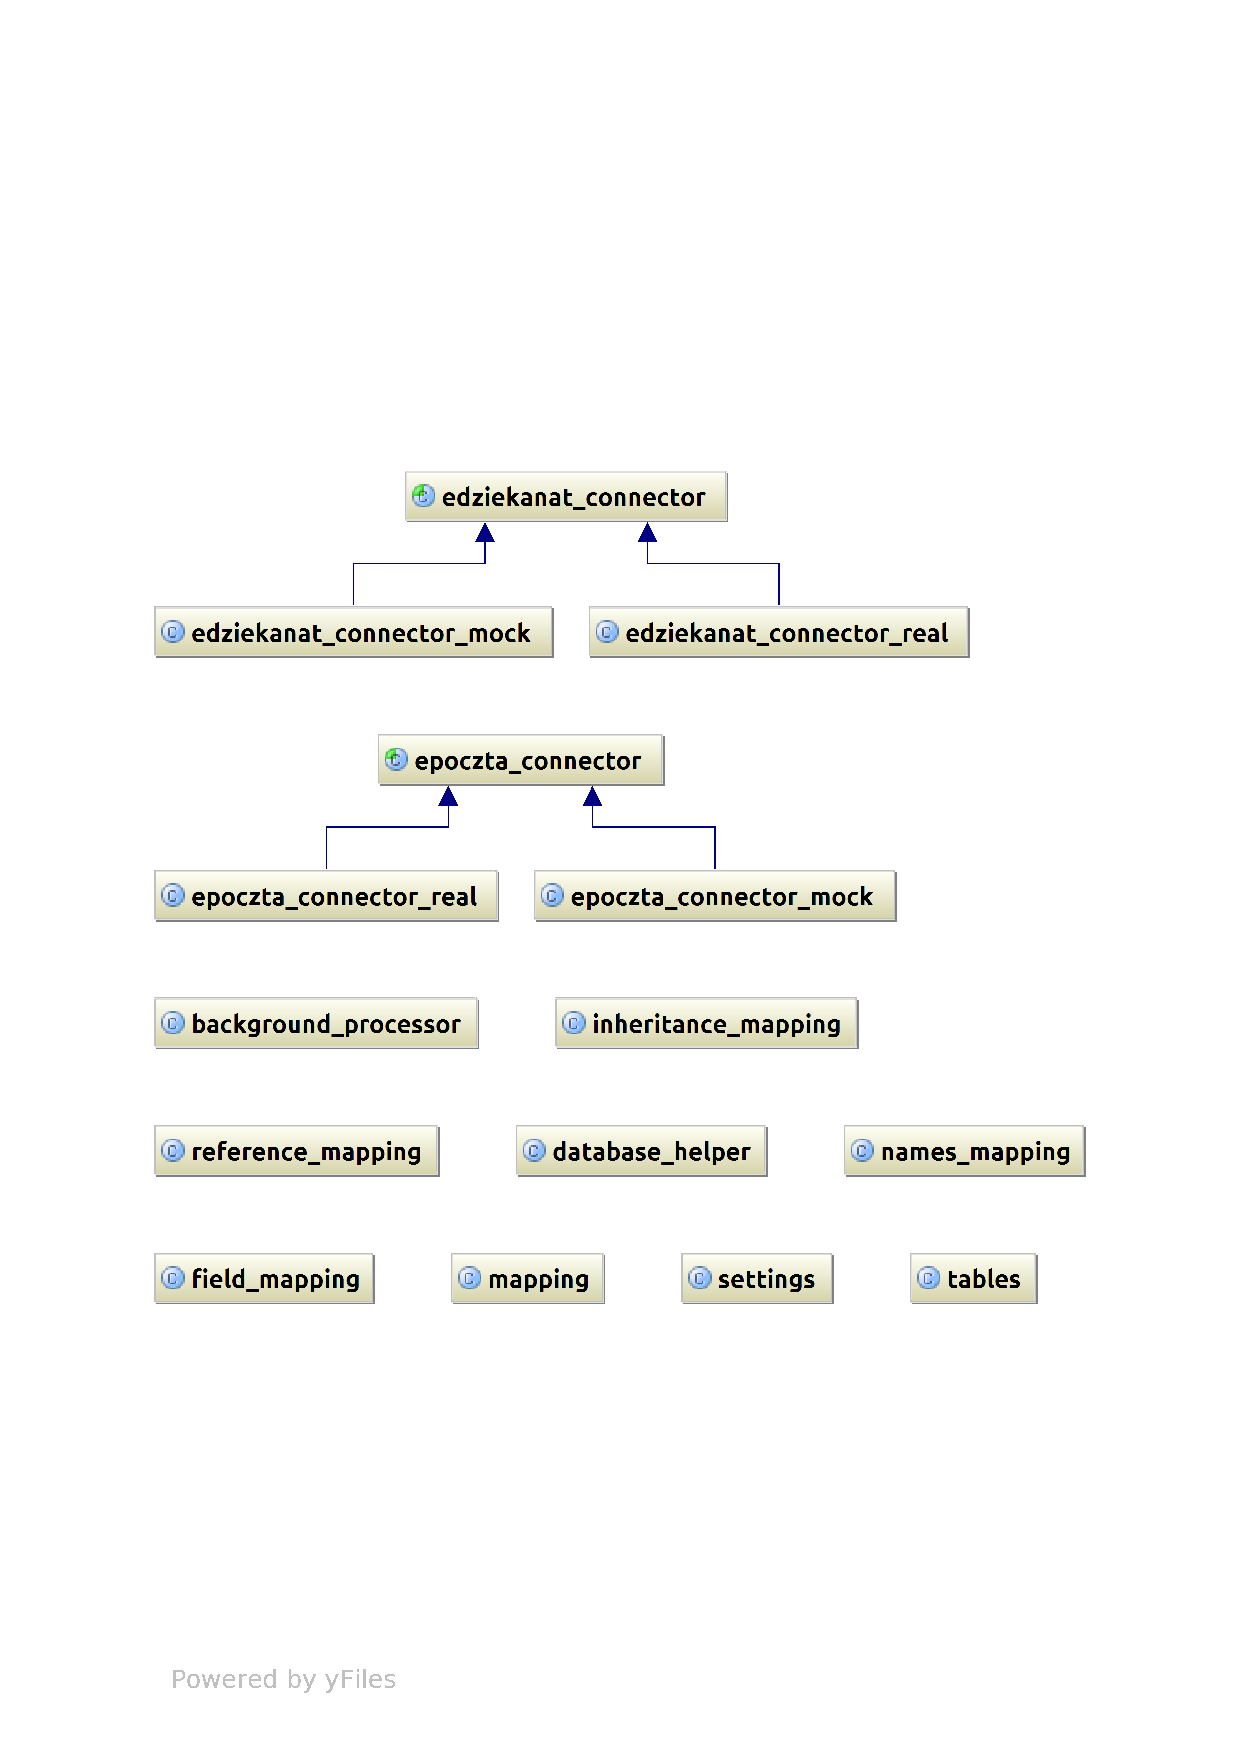
\includegraphics[width=0.8\textwidth]{figures/lw/backend1.pdf} 
\end{center}
\caption{Struktura back-end'u (1)}
\label{fig:back-end1}
\end{figure}

\newpage
\begin{figure}[H]
\begin{center}
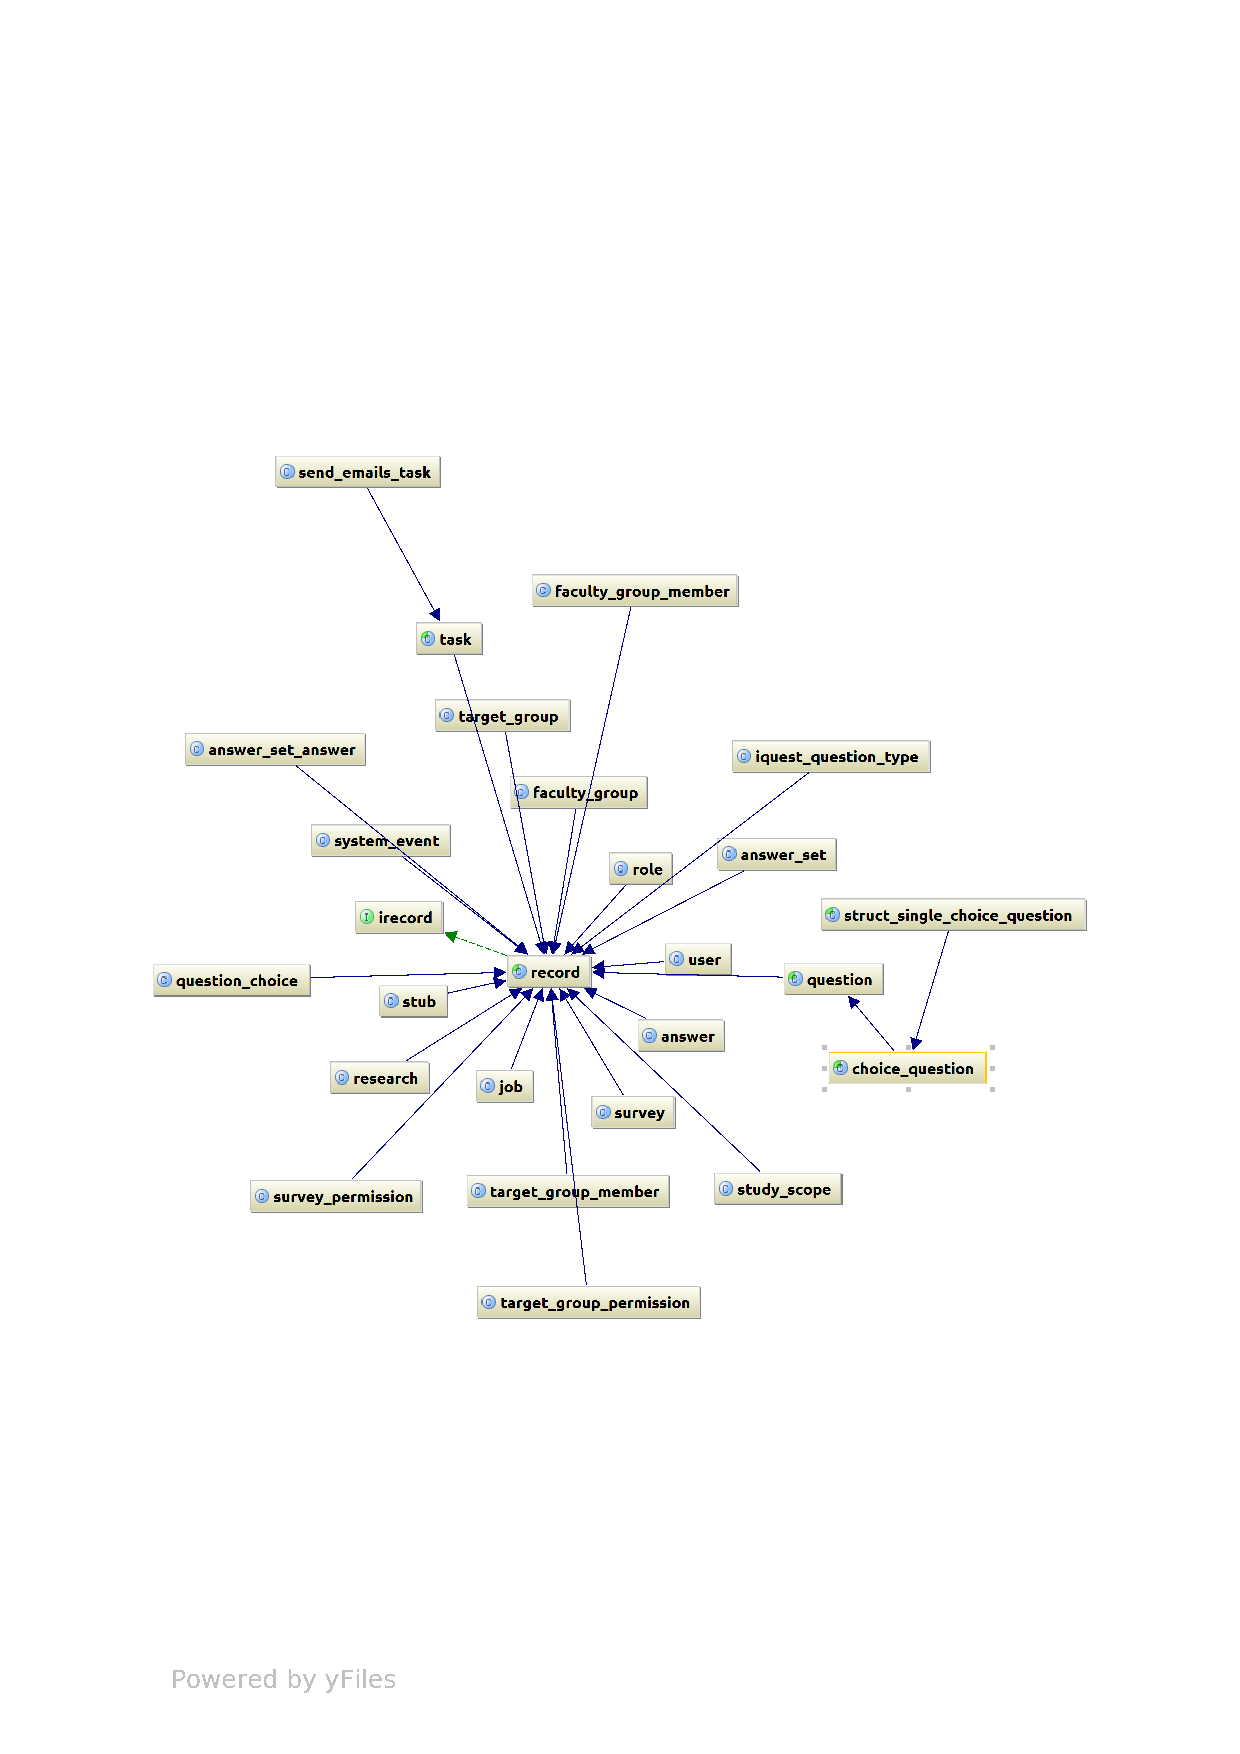
\includepdf{figures/lw/backend2.pdf} 
\end{center}
\caption{Struktura back-end'u (2)}
\label{fig:back-end2}
\end{figure}
\newpage

\subsection{Raporty}
Raporty wykonano korzystając z platformy JasperReports, wykorzystując następujące produkty firmy \emph{Jaspersoft}:

\begin{itemize}
\item \emph{JasperReports Server} (wersja 5.0) -- serwer usług raportowania, na którym przechowywane są przygotowane przez zespół artefakty, w celu umożliwienia generacji raportu osobom dysponującym odpowiednimi uprawnieniami. Wykorzystano następujące funkcjonalności: definiowania źródła danych, raportu, ładowania plików z projektem raportu, zasobami oraz z generacji raportu.
\item \emph{Jaspersoft Studio} (wersja 1.3.2) -- bazowane na Eclipse narzędzie do projektowania raportów. Posłużyło zespołowi do przygotowania projektów raportów w formacie \emph{JRXML}.
\end{itemize}

Kody źródłowe pakietu \emph{JasperReports} są pisane w języku Java. Źródłem danych dla raportu, jest przygotowana przez zespół implementacja interfejsu \emph{ReportDataSourceService} z \emph{API JasperServer}. Źródło danych łączy się z udostępnianymi przez wskazaną instancję systemu \emph{iQuest} usługami zdalnymi, z których otrzymuje informacje o przeprowadzanych badaniach poprzez protokół SOAP. Struktura raportu zależy od typu pytania (otwarte/zamknięte). W przypadku pytań otwartych prezentowana jest lista odpowiedzi. Dla pytań zamkniętych na podstawie pobranych danych generowane są statystyki, które przekazywane są do podraportu w postaci obiektu klasy \emph{JRBeanCollectionDataSource}. W generacji statystyk z danych badań wykorzystano bibliotekę \emph{JoSQL}. Definicja projektu raportu składa się z czterech plików, odpowiadających trzem kolejnych poziomom:
\begin{enumerate}
\item \emph{researches.jrxml} -- raport główny dla badań,
\item \emph{questions.jrxml} -- podraport pytań,
\item \emph{answers\_closed.jrxml} oraz \emph{answers\_open.jrxml} -- podraporty odpowiedzi. zamkniętych i otwartych.
\end{enumerate}
Do generacji namiastek obiektów zdalnych (ang. \definicja{stub}) wykorzystano Apache Axis. Wygenerowane klasy dostosowano tak, by akceptowały obiekty z zadanej instancji \emph{iQuest} oraz dla zmiennej przestrzeni nazw (ang. \emph{namespace}).\\

W trakcie generacji \emph{stub'ów} okazało się, iż definicja usług dla protokołu \emph{SOAP} w języku \emph{WSDL} (\emph{Web Service Description Language}) generowana przez \emph{Moodle} jest niepoprawna. Skorzystano zatem z poprawionej wersji z zewnętrznego źródła (\url{https://github.com/ghigio/moodle-webservice_soapfda}).\\

Dostęp do usług zdalnych definiowanych w \emph{Moodle} zabezpieczono korzystając z mechanizmu generacji tokenu dla wybranego użytkownika. Użytkownik, który z poziomu serwera \emph{Jasper Server} zamierza wygenerować raport, musi znać adres naszego systemu oraz posiadać token dostępu do usługi.

\subsection{Moduły uwierzytelniania}
Korzystając z mechanizmów rozszerzeń \emph{Moodle} zaimplementowano dwa moduły uwierzytelniania, tj.:
\begin{itemize}
\item \emph{eKontoAuthenticationPlugin} -- integruje logowanie przez \emph{eKonto} z naszym systemem,
\item \emph{emailgraduate} -- pozwala absolwentom uczelni na rejestrację z użyciem adresu e-mail.
\end{itemize}

W celu spełnienia wymagań Działu Rozwoju Oprogramowania Politechniki Poznańskiej odnośnie wygaszania sesji użytkownika \emph{eKonto} po zadanym czasie (e.g. 15 min.) zmodyfikowano pliki źródłowe \emph{Moodle}, gdyż dla kodu odnoszącego się do sesji użytkownika \emph{Moodle} nie została przewidziana możliwość rejestracji rozszerzeń. Relacja \emph{user} została rozszerzona o opcjonalne pola związane z \emph{eKonto}, jako że kod odpowiedzialny za manipulację schematem bazy danych nie jest wykonywany podczas instalacji modułu uwierzytelniania, umieszczono go w osobnym module (\emph{ekontodb}). \emph{eKontoAuthenticationPlugin} może być instalowany bez konieczności instalacji \emph{iSurvey}. Podczas jego implementacji korzystaliśmy z dokumentu \emph{Centralne uwierzytelnianie i wymiana danych. Wersja 1.2 (2010.07.06)}.\\

Podczas rejestracji z użyciem naszych modułów użytkownik jest przydzielany do grupy docelowej ,,Absolwenci'', nadawana jest mu też rola respondenta w kontekście \emph{kursu iQuest}. Utworzenie modułu wiąże się z przygotowaniem klasy dziedziczącej z \emph{auth\_plugin\_base}, formularza ustawień, pliku lokalizacji oraz wersji.

\subsection{Moduły dla serwisów zewnętrznych}
\begin{itemize}
\item \emph{ePocztaConnector} -- służy do wysyłania e-maili z serwera Politechniki Poznańskiej,
\item \emph{eDziekanatConnector} -- pobiera i aktualizuje lokalne informacje o grupach dziekańskich, zakresach tematycznych tychże grup oraz ich studentach.
\end{itemize}

\emph{Dział Rozwoju Oprogramowania} udostępnia klienty \emph{eUsług} dla różnych języków, w tym dla \emph{PHP}. Komunikacja z usługami zdalnymi uczelni odbywa się poprzez protokół SOAP. Wyżej wymienione moduły zaimplementowano z wykorzystaniem fabryki obiektów, która w zależności od trybu (testowy/produkcyjny) zwraca obiekt odpowiedniej klasy. Zadania związane z oba modułami są zlecane procesorowi zadań w tle.